\documentclass[10pt,twocolumn,letterpaper]{article}

\usepackage{cvpr}
\usepackage{times}
\usepackage{epsfig}
\usepackage{graphicx}
\usepackage{amsmath}
\usepackage{amssymb}

% Include other packages here, before hyperref.

% If you comment hyperref and then uncomment it, you should delete
% egpaper.aux before re-running latex.  (Or just hit 'q' on the first latex
% run, let it finish, and you should be clear).
\usepackage[breaklinks=true,bookmarks=false]{hyperref}

\cvprfinalcopy % *** Uncomment this line for the final submission

\def\cvprPaperID{****} % *** Enter the CVPR Paper ID here
\def\httilde{\mbox{\tt\raisebox{-.5ex}{\symbol{126}}}}

% Pages are numbered in submission mode, and unnumbered in camera-ready
%\ifcvprfinal\pagestyle{empty}\fi
\setcounter{page}{1}
\begin{document}

%%%%%%%%% TITLE
\title{Recognizing Strong Gravitational Lenses}

\author{Chris Davis\\
{\tt\small cpd@stanford.edu}
% For a paper whose authors are all at the same institution,
% omit the following lines up until the closing ``}''.
% Additional authors and addresses can be added with ``\and'',
% just like the second author.
% To save space, use either the email address or home page, not both
\and
Andrew McLeod\\
{\tt\small ajmcleod@stanford.edu}
}

\maketitle
%\thispagestyle{empty}

% %%%%%%%%% ABSTRACT
% \begin{abstract}
%    The ABSTRACT is to be in fully-justified italicized text, at the top
%    of the left-hand column, below the author and affiliation
%    information. Use the word ``Abstract'' as the title, in 12-point
%    Times, boldface type, centered relative to the column, initially
%    capitalized. The abstract is to be in 10-point, single-spaced type.
%    Leave two blank lines after the Abstract, then begin the main text.
%    Look at previous CVPR abstracts to get a feel for style and length.
% \end{abstract}

%%%%%%%%% BODY TEXT
\section{Introduction}

A consequence of Einstein's Theory of General Relativity is that mass bends the
path of light. Most of the time the deflections are very small; the original
'gravitational lens' that tested the veracity of Einstein's theory in the years
after the first world war was the sun, which deflected light from stars behind
it only a few seconds of arc. However, when light passes through a particularly
deep gravitational potential (say, near the center of the dark matter halo of a
galaxy cluster), the deflections can be particularly large, resulting in
brilliant arcs and multiple images. These strong deflections due to light
passing through a deep gravitational potential are termed strong gravitational
lenses.

The very existence of these potentials acts as a verification of the Theory of
General Relativity, but they can also be used for much more. Strong
gravitational lenses are one of the few ways to directly probe the distribution
of dark matter, a particle (or possibly family of particles) that does not emit
electromagnetic radiation but does have mass and hence interacts
gravitationally with normal baryonic matter. This allows us to tally the mass
of the largest gravitationally-bound structures in the universe, galaxy
clusters, which can give us insight into the formation history of these massive
objects. In this way, strong gravitational lenses can then tell us something
about the expansion history of the universe, by setting limits on how massive
the most massive objects in the universe can be. The properties of the bent
light itself can also say much about that expansion history. When an object is
strongly-lensed into multiple images, each image travels a different span of
space and time. When an object does not vary much with time, these different
path lengths have no practical import. However, if the object varies
appreciably quickly (say it is a distant supermassive black hole at the center
of a galaxy whose accretion disk emits high-energy radiation at varying rates)
then these different path lengths can be used to pin down the rate of expansion
of the universe.

Unfortunately, for how useful strong gravitational lenses are, they are also
extremely rare. A next generation optical survey like the Large Synoptic Survey
Telescope can expect to find only ten thousand lenses in the whole sky, while
it will find ten billion galaxies. Currently in astronomy there are only order
hundreds of strong gravitational lenses known, mostly discovered by 'eyeball
squads' of graduate students. The small number means that target criteria must
be somewhat broad in order to maintain a relatively high completeness. Using
reasonable target criteria to find strong lenses such as looking only at
massive galaxies still means that nearly ten million objects will need to be
inspected in the next generation in order to find those ten thousand lenses. A
team of ten graduate students could expect to spend about 14 years looking at
these objects. Computer algorithms are not much better: most current machine
learning algorithms are woefully-underpowered for this task, and generally have
poor completeness or poor purity -- and often poor both. Additionally, some
algorithms are better at finding some types of lenses than others; some
perform well on the brilliant arcs, but poorly on the multiply-imaged objects,
or vice versa. New algorithms need to be developed to find more strong
gravitational lenses, and more strong lenses need to be found to power these
algorithms.

{\sc Space\,Warps}\xspace (Marshall et. al, in prep.) is a citizen-science
initiative designed to overcome these two problems. The program has users
examine images from the Canada-France-Hawaii Telescope Legacy Survey (CFHTLS)
and vote on where they see lenses. Users are also assessed and trained with
simulated lenses and known empty fields. By having thousands of users analyze a
survey for short amounts of time each, it is hoped that a more complete sample
of lenses can be discovered, which can then be fed into lens-finding algorithms
to further improve their performance.

\begin{figure*}[!ht]
\begin{minipage}[b]{0.24\linewidth}
\centering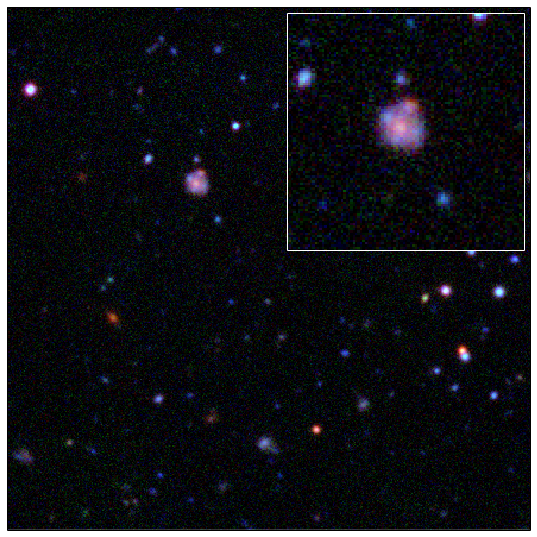
\epsfig{file=figs/gallery/0.png,width=\linewidth,angle=0,clip=}
\end{minipage} \hfill
\begin{minipage}[b]{0.24\linewidth}
\centering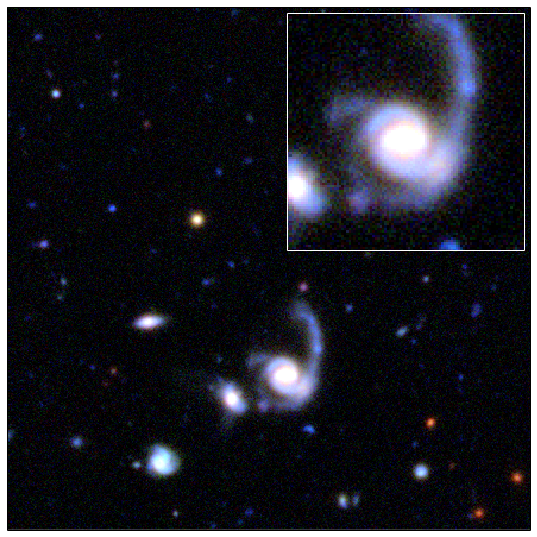
\epsfig{file=figs/gallery/1.png,width=\linewidth,angle=0,clip=}
\end{minipage} \hfill
\begin{minipage}[b]{0.24\linewidth}
\centering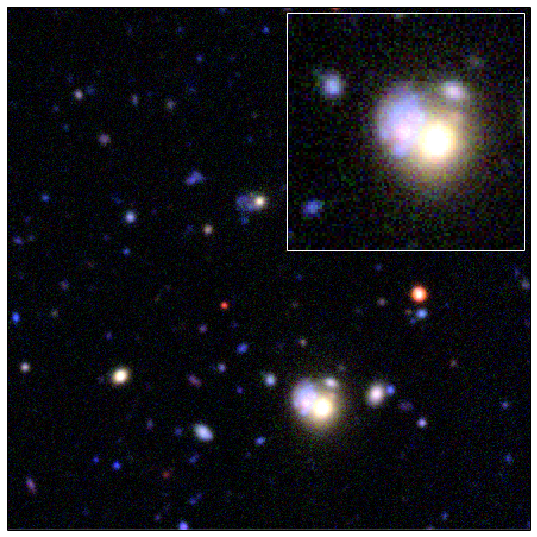
\epsfig{file=figs/gallery/2.png,width=\linewidth,angle=0,clip=}
\end{minipage} \hfill
\begin{minipage}[b]{0.24\linewidth}
\centering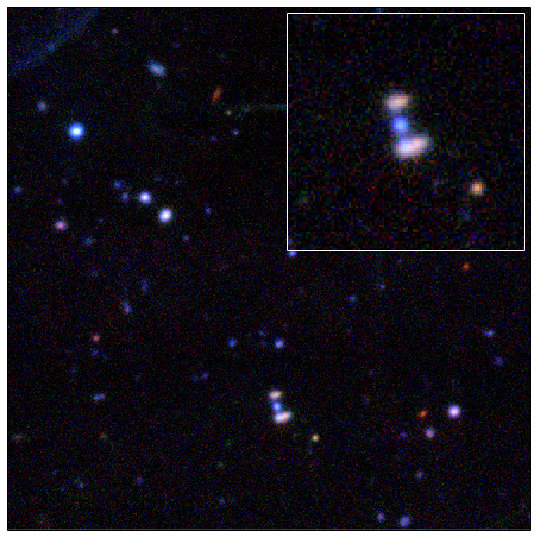
\epsfig{file=figs/gallery/3.png,width=\linewidth,angle=0,clip=}
\end{minipage} \hfill
  \caption{Typical Space Warps duds. Insets indicate regions where volunteers typically
  clicked.}
  \label{fig:duds}
\end{figure*}

\begin{figure*}[!ht]
\begin{minipage}[b]{0.24\linewidth}
\centering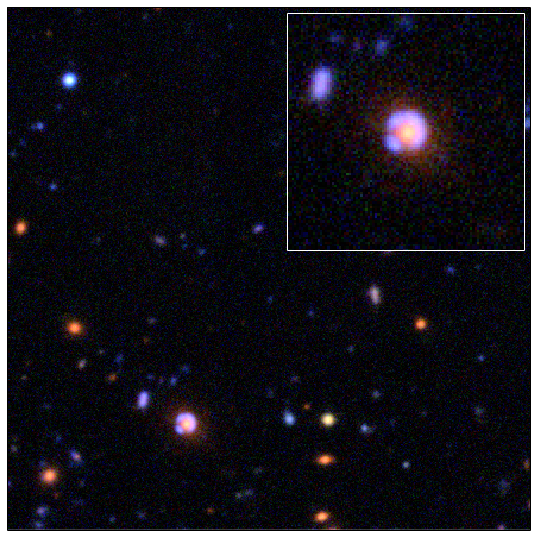
\epsfig{file=figs/gallery/4.png,width=\linewidth,angle=0,clip=}
\end{minipage} \hfill
\begin{minipage}[b]{0.24\linewidth}
\centering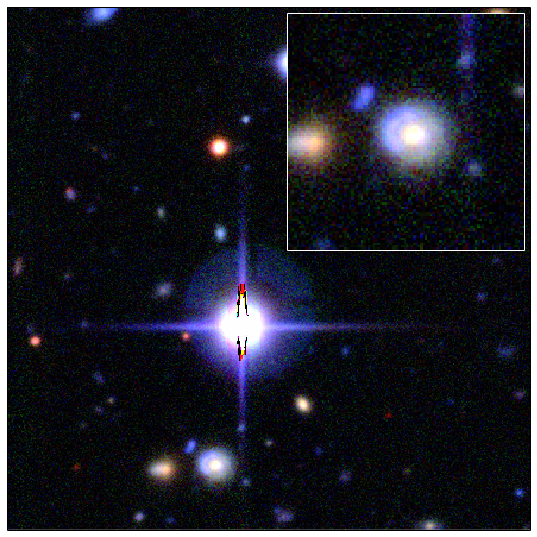
\epsfig{file=figs/gallery/5.png,width=\linewidth,angle=0,clip=}
\end{minipage} \hfill
\begin{minipage}[b]{0.24\linewidth}
\centering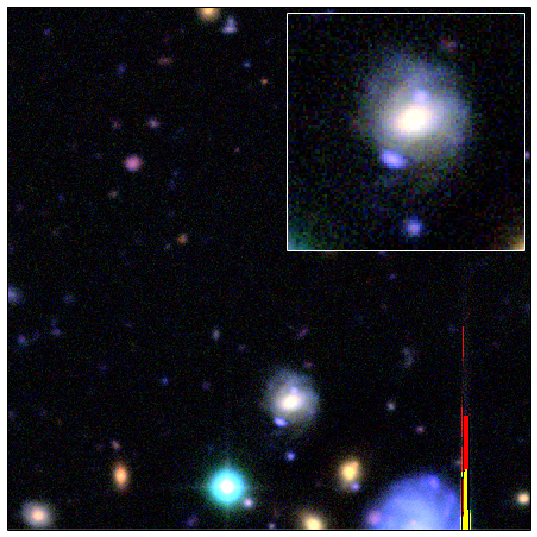
\epsfig{file=figs/gallery/6.png,width=\linewidth,angle=0,clip=}
\end{minipage} \hfill
\begin{minipage}[b]{0.24\linewidth}
\centering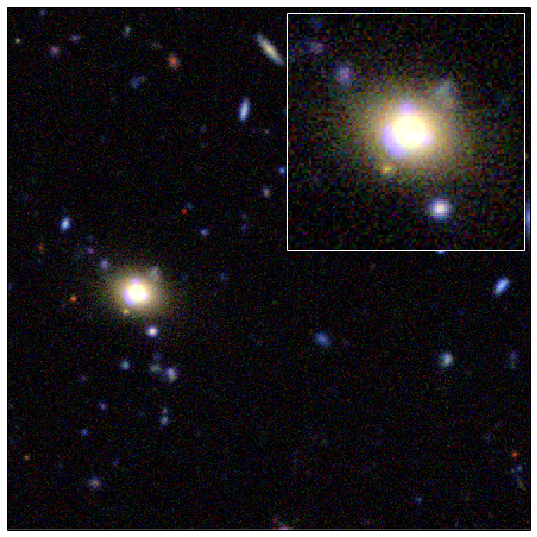
\epsfig{file=figs/gallery/7.png,width=\linewidth,angle=0,clip=}
\end{minipage} \hfill
  \caption{Typical sims. Insets indicate the location of the lens in the
  image.}
  \label{fig:sims}
\end{figure*}

%-------------------------------------------------------------------------
\section{Problem Statement}

In this project we will use images collected by the Canada-France-Hawaii
Telescope Legacy Survey to analyze how Convolution Neural Networks can improve
automated detection of strong lens systems. We will also assess the performance
of citizen scientists by comparing our results to them. From other graduate
work (but not coursework), we have the locations and categories of around one
hundred and twenty known strong lenses, three thousand large fields verified to
contain no strong lenses, six thousand simulated strong lenses, and several
thousand classifications by citizen-scientists of other potential strong lens
systems.  These will form the core of our training and testing datasets; our
metric will be how well a CNN correctly identifies known and simulated lenses
and non-lens systems.

We would like to examine the following questions:
\begin{itemize}
\item{ Do we have enough data to reasonably train and test a CNN? Can we get
       around this by artificially inflating the data, e.g. by adding rotated
     images?}
\item{ What processing needs to be done on the data? What kind of scaling of
       pixel data is appropriate for automated detection? Should we compress
     the five different 'colors' to a smaller number of dimensions?}
   \item{ How do citizen-scientists do compared with this automated system?}
   \item{Can we use the results of citizen-scientists to train the CNN?}
\item{What sets of classifications are needed? Are we better served sticking
       to 'lens' and 'not lens', or should we use several classification
       categories ('lensed arcs', 'lensed multiple images', 'non-lens pixel
     noise')?}
\end{itemize}


%-------------------------------------------------------------------------
\section{Technical Approach}

From approximately 12000 fields of $440\times440\times3$ fields, we have
constructed approximately 30000 cutouts sized $96\times96\times3$. These cutouts
are selected based on where citizen scientists clicked, on the theory that both
'correct' and 'incorrect' selections provide useful information about the
characteristics of gravitational lenses. In general, we have access to two
broad classes of images: 'training' and 'test' images. The 'training' images
include fields that were verified in advance to not contain any lenses as well
as simulated lensed galaxies, quasars, and clusters. Many of the simulated
objects are over-exaggerated and extremely obvious, but we also have access to
a second 'refinement stage' of the project, where much harder simulations were
given to users. The 'test' images are the fields that citizen scientists
viewed, assessing whether a lens was in the field or not. In these 'test'
images are 120 known strong gravitational lens systems, which are also included
in this set. (The project confirms roughly half of these known lenses for
reasonable definitions of completeness and purity.) For all the images we also
have an associated probability that the project would evaluate that system as
containing a lens.

It is clear that we do not have enough data. Luckily, we also know that our
lens objects must obey certain symmetry properties, so it is quite easy to
augment our data. For example, we know that strong lens systems should be
independent of rotations as well as small amounts of stretching and
translation, so our data can be augmented by applying those transformations to
our images.

We plan to train a classifier on this data using two different methods. First,
we will code our own convolutional net in python using theano. Second, we will
apply transfer learning techniques to train on a convolutional net galaxy
morphology classifier, which has graciously been made available to us by Ryan
Keisler and which achieved 7th place in the 2014 Galaxy Zoo Kaggle competition.
This classifier runs $96\times96$ images through 3 convolutional layers and 2
fully-connected layers and predicts a galaxy to have one of 37 enumerated
morphologies. We plan to train our classifier on top of the first
fully-connected layer, which has 500 neurons.


%-------------------------------------------------------------------------
\section{Intermediate/Preliminary Results}

We have created the cutouts of our images from the catalogs.
We have begun constructing our own convolutional network with two
convolutional/max-pool layers and two fully-connected layers. Although we have
not yet trained on our images, we can load these images and run them
through our initialized classifier. Figures~\ref{fig:duds} and
\ref{fig:sims}\xspace show example fields with cutouts inlaid.

% {\small
% \bibliographystyle{ieee}
% \bibliography{egbib}
% }

\end{document}
